\documentclass[a4paper, 12pt]{report}

%====================== PACKAGES ======================

\usepackage[english]{babel}
\usepackage[utf8x]{inputenc}
%immage psitioning management
\usepackage{float}
\usepackage{amsmath}
\usepackage{graphicx}
\usepackage[colorinlistoftodos]{todonotes}
\usepackage{url}
%for informations on a compiled PDF file and external/internal links
\usepackage{hyperref}
%for array layout setup
\usepackage{array}
\usepackage{tabularx}
%to use \floatbarrier
%\usepackage{placeins}
%\usepackage{floatrow}
%interline spacing
\usepackage{setspace}
%modify abstract layout
\usepackage{abstract}
%font and margins of the document
\usepackage[T1]{fontenc}
\usepackage[top=2cm, bottom=2cm, left=2cm, right=2cm]{geometry}
%For images galerie
\usepackage{subfig}
\usepackage[numbers]{natbib}%numbers
\usepackage{doi}

%====================== INFORMATION ET RULESS ======================

%rajouter les numérotation pour les \paragraphe et \subparagraphe
\setcounter{secnumdepth}{4}
\setcounter{tocdepth}{3}

\hypersetup{	
	colorlinks = true,
	allcolors = magenta,
	linkcolor = .,
	citecolor = magenta,%
	anchorcolor = .,
	%
	%
						% Information sur le document
pdfauthor = {Esteban Marquer,
			Prerak Shrivastava},			% Auteurs
pdftitle = {Anomaly detection with deep learning models -
			Bibliography report},			% Titre du document
pdfsubject = {Bibliography report},		% Sujet
%pdfkeywords = {Tag1, Tag2, Tag3, ...},	% Mots-clefs
pdfstartview={FitH}}					% ajuste la page à la largueur de l'écran
%pdfcreator = {MikTeX},% Logiciel qui a crée le document
%pdfproducer = {}} % Société avec produit le logiciel

%======================== DEBUT DU DOCUMENT ========================

\begin{document}

%régler l'espacement entre les lignes
\newcommand{\HRule}{\rule{\linewidth}{0.5mm}}

%page de garde
\begin{titlepage}
\begin{center}

% Upper part of the page. The '~' is needed because only works if a paragraph has started.

\includegraphics[width=0.35\textwidth]{./logo}~\\[1cm]

\textsc{\LARGE Université ou Entreprise}\\[1.5cm]

\textsc{\Large }\\[0.5cm]

% Title
\HRule \\[0.4cm]

{\huge \bfseries Nom du Projet\\
Sujet du Projet \\[0.4cm] }

\HRule \\[1.5cm]

% Author and supervisor
\begin{minipage}{0.4\textwidth}
\begin{flushleft} \large
\emph{Auteur:}\\
Premier \textsc{Auteur}\\
Deuxième \textsc{Auteur}\\
Troisième \textsc{Auteur}\\
Quatrième \textsc{Auteur}
\end{flushleft}
\end{minipage}
\begin{minipage}{0.4\textwidth}
\begin{flushright} \large
\emph{Client:} \\
Prénom \textsc{Nom}\\
\emph{Référent:} \\
Prénom \textsc{Nom}
\end{flushright}
\end{minipage}

\vfill

% Bottom of the page
{\large \today}

\end{center}
\end{titlepage}

%page blanche
\newpage
~
%ne pas numéroter cette page
\thispagestyle{empty}
\newpage

%\renewcommand{\abstractnamefont}{\normalfont\Large\bfseries}
%\renewcommand{\abstracttextfont}{\normalfont\Huge}

\begin{abstract}
\hskip7mm

\begin{spacing}{1.3}

Lorem ipsum dolor sit amet, consectetur adipiscing elit. Sed non risus. Suspendisse lectus tortor, dignissim sit amet, adipiscing nec, ultricies sed, dolor. Cras elementum ultrices diam. Maecenas ligula massa, varius a, semper congue, euismod non, mi. Proin porttitor, orci nec nonummy molestie, enim est eleifend mi, non fermentum diam nisl sit amet erat. Duis semper. Duis arcu massa, scelerisque vitae, consequat in, pretium a, enim. Pellentesque congue. Ut in risus volutpat libero pharetra tempor. Cras vestibulum bibendum augue. Praesent egestas leo in pede. Praesent blandit odio eu enim. Pellentesque sed dui ut augue blandit sodales. Vestibulum ante ipsum primis in faucibus orci luctus et ultrices posuere cubilia Curae; Aliquam nibh. Mauris ac mauris sed pede pellentesque fermentum. Maecenas adipiscing ante non diam sodales hendrerit. Ut velit mauris, egestas sed, gravida nec, ornare ut, mi. Aenean ut orci vel massa suscipit pulvinar. Nulla sollicitudin. Fusce varius, ligula non tempus aliquam, nunc turpis ullamcorper nibh, in tempus sapien eros vitae ligula. Pellentesque rhoncus nunc et augue. Integer id felis. Curabitur aliquet pellentesque diam. Integer quis metus vitae elit lobortis egestas. Lorem ipsum dolor sit amet, consectetuer adipiscing elit. Morbi vel erat non mauris convallis vehicula. Nulla et sapien. Integer tortor tellus, aliquam faucibus, convallis id, congue eu, quam. Mauris ullamcorper felis vitae erat. Proin feugiat, augue non elementum posuere, metus purus iaculis lectus, et tristique ligula justo vitae magna. Aliquam convallis sollicitudin purus. Praesent aliquam, enim at fermentum mollis, ligula massa adipiscing nisl, ac euismod nibh nisl eu lectus. Fusce vulputate sem at sapien. Vivamus leo. Aliquam euismod libero eu enim. Nulla nec felis sed leo placerat imperdiet. Aenean suscipit nulla in justo. Suspendisse cursus rutrum augue. Nulla tincidunt tincidunt mi. Curabitur iaculis, lorem vel rhoncus faucibus, felis magna fermentum augue, et ultricies lacus lorem varius purus. Curabitur eu amet.

\end{spacing}
\end{abstract}


\tableofcontents
\thispagestyle{empty}
\setcounter{page}{0}
%ne pas numéroter le sommaire

\newpage

%espacement entre les lignes d'un tableau
\renewcommand{\arraystretch}{1.5}

%====================== INCLUSION DES PARTIES ======================

~
\thispagestyle{empty}
%recommencer la numérotation des pages à "1"
\setcounter{page}{0}
\newpage

\chapter*{Introduction}
\addcontentsline{toc}{chapter}{Introduction}

Logs are an important part of any computer ecosystem today but, to understand and make future decision on these logs is an hard and important task these days.
Deep Learning has emerged as a key player to complete this motto due to its state of the art performance on various major tasks related to anomaly detection. Among those tasks, there is intrusion detection, denial of service (DoS) attack detection, hardware and software system failures detection, and malware detection. However, in recent years deep learning is often regarded as black box due to the need of understanding very hard mathematical complexity and algorithms, and the lack of direct and simple interpretability.

Our project centers on anomaly detection in large amounts of system logs, with very few occurrences of said anomalies in available data. The project thus concentrates on realizing a top notch predictive system, used to model the normal behavior of the logs. Deviations from that behavior can be considered anomalies.

Based on those observations, we try to explain in this work a major deep learning architecture, the DAN (Deep Averaging Network), which we are using in our project and is also a state of the art architecture for major Natural Language Processing (NLP) tasks.
Apart from this work we also shed some light on other state of the art technique like RNN (Recurrent Neural Network) using attention mechanism, and LSTM (Long and Short Term Memory) Networks.
We plan to demonstrate our model’s performance and to illustrate its interpretability using the Los Alamos National Laboratory (LANL) cyber-security dataset in the upcoming parts. We will present that dataset along with our main dataset of industrial data from the PAPUD project in the last part of the report.



%\chapter{[WIP] Anomaly detection in system logs}


 
\chapter{Different artificial neural network architectures and techniques}

Currently, in the literature we can find a variety of neural network architectures. By "architecture" we mean the major structure of a neural network (the way the neurons are organized in layers and how these layers are connected for example). We will present here some of those architecture that can be used for anomaly detection in system logs, along with techniques used along those models.

Also, as current literature shows increasingly \cite{rnn_attention_lanl}, character-level models achieve similar performance than word-level models, while managing out-of-domain data way better (it is way less likely to encounter an unknown character than to encounter a new word).

\section{Multi-layer Perceptron / Fully Connected Layers}
The first model we ought to present is the multi-layer perceptron \cite{deep_learning_book}, a very simple neural network architecture.
It is composed of multiple layers of neurons, with every neuron of a layer connected to all the neurons of the next layers. Between each pair of layers an activation function, also called non-linearity, is added.

Even if its basic concept dates of the 80s \cite{mlp} and is far from being state of the art, it is still used in more complex architectures such as the Deep Averaging Neural Network.

\section{Preprocessing}
"Preprocessing" designates all the operations applied on the data to filter inappropriate data and adapt its representation to obtain the best quality data as input for the model.

For example, in \cite{lstm_cluster} various preprocessing techniques are used on the input log lines data. In particular, they use a clustering technique on the raw text from multiple log sources to extract specific information from the logs and generate sequences that it be fed into a Long and Short Term Memory Network (LSTM, described \autoref{sec:lstm}) network. By using such handcrafted feature extraction processes, they are able to improve the performance of their model by removing unnecessary information from the original data.

However, handcrafted feature extraction is costly to produce, and may remove potentially useful information.

In contrast to \cite{lstm_cluster}, our algorithm works almost directly on the logs, with the only preprocessing being the mapping of all the characters to numbers through an automatically generated dictionary.
We also normalize the size of each log line, by padding them with a specific character or removing the excess characters.
For reference, in \cite{rnn_attention_lanl} they need an additional step of tokenization using know delimiters because they are also using words and not only characters.

\section{Embeddings}
Various deep learning NLP models use word or character embeddings \cite{pooling_simple,deep_learning_book}. They are a kind of mapping that gives a way to represent efficiently the words (or character), instead of using 1-hot tensors (tensors of zeros, except for the cell corresponding to the word which is one). The mapping is either pre-trained or learned alongside the model. This way, a full dictionary can be represented with almost no loss in information in less than 200 dimensions (instead of one dimension per word). Quite the opposite in fact, as forcing a dimensionality reduction force the embedding to learn similarity between words.

\section{Attention Models}
Recently, a group of researchers have modified a LSTM (see \autoref{sec:lstm}) and are now using it with attention mechanisms in order to capture long term dependencies on the system logs \cite{rnn_attention_lanl}.
The attention mechanisms allows us to get some insight about what factors are affecting the model’s decision, by observing which elements are selected by the attention weights. Attention mechanisms also enable to select recover information from a context, like previously seen elements, thus allowing the capture of long term dependencies.
But, in contrast, in our model we did not use any kind of attention mechanism but rather kept it simple, because of the complexity of attention mechanisms ans the high time and resource cost they induce. To get the long term dependencies between the log lines is currently not in the scope of our project, but is rater planned as way later step in the process to answer the problematic.

\section{Order-sensitivity of the model}
One last point of interest, that will directly lead us to the architecture we will use, is whether our model should be sensitive to the order of the elements in the input data or not. This divides the architectures in two families: unordered and syntactic. Unordered means that we convert the text to a bag of word embeddings, without a care for the order of the elements, while syntactic keeps order of the input text and is thus able to discover syntactic information.

For example with sentiment analysis, given a sentence like “The movie was entertaining but i don't like it very much” an unordered model like NBOW (see \autoref{sec:nbow}) will have trouble dealing with the negation in “don't like”, and thus will most probably return a positive label, which is a mistake. Syntactic aware models, like RNNs and LSTMs (see \autoref{sec:lstm}), or CNNs (see \autoref{sec:cnn}), are way more likely to handle such things.

\subsection{Recurrent Neural Network (RNN) and Long and Short Term Memory Neural Network (LSTM)\label{sec:lstm}}
RNN’s architecture of is made in such a way that it can keep track of the phrase or the words  that have appeared in the beginning of the sentence and thus can make final decision according to it. It has proven to be very efficient in many NLP applications \cite{rnn_attention_lanl,UnreasonableRNN}.
However, with this advantage also comes the disadvantage of having a large training time and hardware use.
The main reason is that the non-linearities and matrix/tensor products at each node of the parse tree of a RNN are expensive, especially as model dimensionality increases. 
It also seems RNNs can sometime also struggle to deal with out of domain data.

LSTMs are a variant of RNNs, more complex and more powerful, but they also requires an even larger amount of training time and computations.
They are considered one of the state of the art in the domain \cite{LSTM}.

\subsection{Convolutional Neural Network (CNN) \label{sec:cnn}}
However, Y. Kim in his paper \cite(cnn-2) shows that Convolutional Neural Network (CNN) can deal with both the dependency problem and the out of domain data, while giving effective results with low training time and hardware constraints.
The CNN architecture has proven its efficiency with image processing, but it still proves to be very efficient with text.
A CNN uses a sliding window (also called kernel) that run through the data to extract local information and process it.
CNNs can have various channels with different kernel sizes, which give very good results because those various channels can capture different important information on different scales on a single given input sentence. For example, one channel can capture information about the word structure while another can capture grammatical information.
However, the presence of multiple channels with various sliding windows, while composed of very simple operations, cause the computational cost to increases for large amounts of data (especially if we compare the training time with the one of a DAN (see \autoref{sec:dan})).
\cite{deep_learning_book, cnn-1}

\subsection{Neural Bag of Word (NBOW) \label{sec:nbow}}
The NBOW model just contains 4 major steps that are defined as follows \cite{bow}:
\begin{enumerate}
	\item the conversion of text into tokens
	\item the conversion of tokens into embeddings
	\item the model average out the embedding which produces a vector “z”
	\item it performs a softmax (operation that transform a set of values into a probability distribution) on “z” to get the probability of the labels
\end{enumerate}

During training, we apply the cross-entropy function to calculate the error and back-propagate the error throughout the model.
Due to being composed of very simple functions (embedding, averaging, softmax), the NBOW model is quite simple and fast to train.

We have explained NBOW model here because it will serve as a baseline for DAN model because DAN is simply a modification of NBOW model

\subsection{Deep Averaging Neural Network \label{sec:dan}}
The Deep Averaging Network \cite{dan_1, dan_2} model works in 3 simple steps that are described as follows 
\begin{enumerate}
	\item take the vector average of the embeddings associated with an input sequence of tokens
	\item pass that average through one or more feed-forward layers
	\item perform a (linear) classification on the final layer representation (in our project, this step is replaced by the generation of the next log line)
\end{enumerate}

An advantage of the DAN model is its high processing speed.
Deep Averaging Network is a modification of an NBOW (Neural Bag Of Words Model), by adding the linear classification step to the model.

\section*{Choice of DAN}

Although syntactic composition is very useful to obtain powerful models for example with LSTM, it requires a long training and expensive computations thus slows down the process. In our case, the dataset is very huge so such costs aren't really affordable.
Even if CNN offer a less thorough syntactic composition support, they still require a larger amount of resources than DAN. However, with CNN the cost seem more affordable.
Furthermore, DAN network can also be trained on various types of data without the need of large amount of pre-processing and also can be applied to the data with high syntactic variance.


% DAN part ?
\chapter{In-depth description of the Deep Averaging Network (DAN)}

\section{Internal structure of the DAN}
As DAN is a modification of an NBOW model, with an additional perceptron between the average tensor and the softmax. It is a feed-forward neural network (it does not use recurrency nor convolutions), and each layer of the perceptron learns a more confined information of input sequence than the previous layer.

To be more concrete, take s1 as the sentence "I really loved Waffles performance in Belgium" and generate s2 and s3 by replacing "loved" with "liked" and then again by “did not like”, then you will see that the embedding average of s1 and s2 is quite similar to each other, while the average for s3 is only a little bit different from the previous two. However, the meaning of s3 is really different from the other two.
The  hidden layers in the DAN are able to amplify those "small but meaningful differences in the word embedding average" \cite{dan_1}, allowing it to achieve state of the art performance with very little computational cost.

The addition of numerous 2-3 feed forward layers allows to increase the depth in the model and also allows to capture subtle variation in the input better than NBOW and computing each layer in feed forward layer is just a simple matrix multiplication. In practice the training time of DAN and NBOW is more or less the same.

So, instead of directly giving this output to the final layer we compute and give it to numerous layers in between as depicted in the \autoref{fig:1}. The figure also shows the obvious scalability advantage of DAN over RNN, because the number of computations increase according to the size of the input data while the averaging in DAN absorbs the size variation.

\begin{figure}[!h]
	\begin{center}
		%taille de l'image en largeur
		%remplacer "width" par "height" pour régler la hauteur
		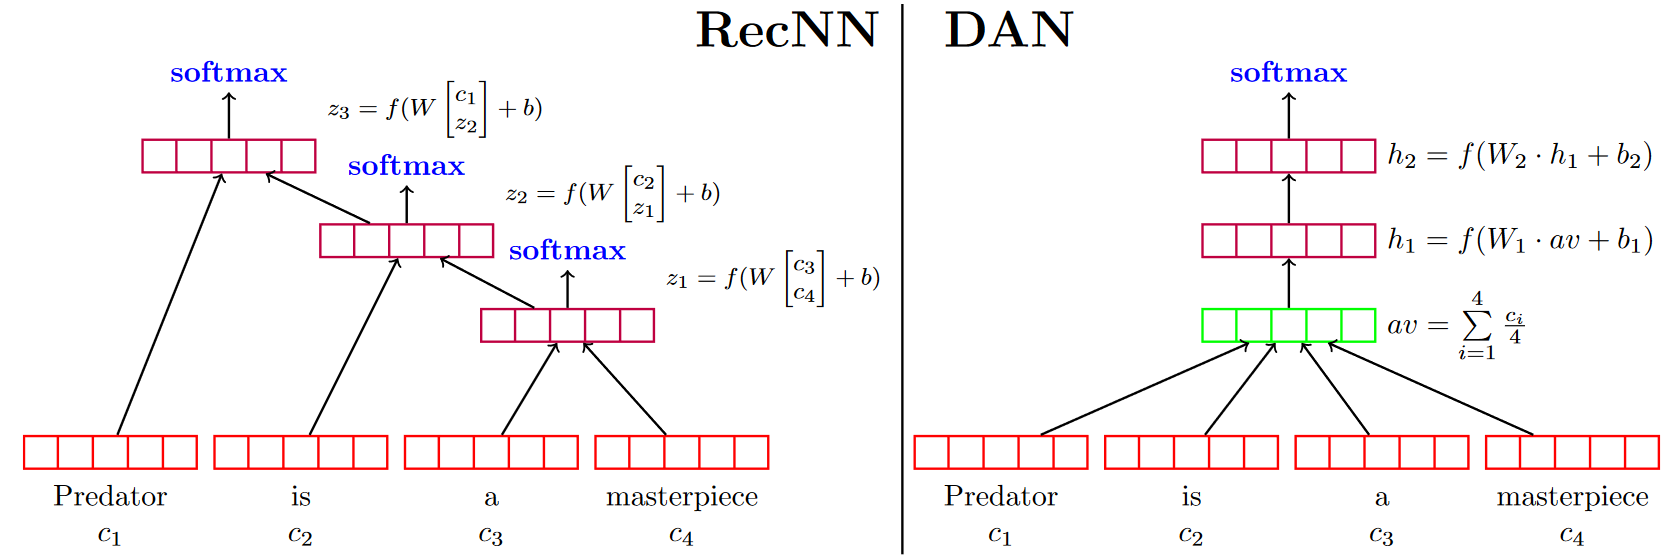
\includegraphics[width=15cm]{img/rnn_dan}
	\end{center}
	%légende de l'image
	\caption{Comparison of the DAN model system with a basic RNN\cite{dan_1}\label{fig:1}}
\end{figure} 

\section{Improving Performances}
To improve the performance of DAN network we have used we can perform dropout on input word sequences by randomly dropping a word in a sentence by a some defined probability. The basic motto of dropout is that it prevents overfitting of the data in the model, by randomly removing part of the data, thus artificially increasing the number of different examples.
In DAN model we can drop word tokens or part of the embedding average. Using this method our input sequence to the model see different token sequence for each input X. However, dropout may also drop words or characters which are really necessary for  the analysis of the input sequence. But most of time this method improves the performance of the model.
We can note that the dropout technique work well with DAN models although it can alter and deteriorate the results if applied to other models like RNN or LSTM.

\section{DAN For Predictive Maintenance}
In our project we are using the DAN model to predict the next occurring system log in a sequence of many logs. As described in the upcoming sections, we have a very large data set (comparatively to the usual datasets used in deep learning). Compared with other state of the art architectures like the RNN or LSTM, which concentrate on achieving high performance with a low amount of data, the DAN would give us equivalent or better performance, while maintaining a very low training time necessary to draw the most of the amount of available data.
DAN can also magnify small and meaningful differences from the different logs. Another interesting feature of, the DAN is its ability to incorporate out-of-domain data which is useful to maintain a stable predictive ability.


\chapter{Corpora used}

\section{The original corpora: the industrial dataset from the PAPUD project}
Just a few lines to present the industrial corpus

The data from the PAPUD project is given to us by industrial partners of the project (BULL-ATOS). It is a set of system log files from their servers, which in total amount to more than 400GiB of compressed data; we are currently using a small subset of this data for our model.

The data from that dataset is confidential. Thus, the example we present in \autoref{tab:indu} has been altered.


\begin{figure}[!h]
	\begin{center}
		
		\begin{tabularx}{.9\textwidth}{|X|X|}
			\hline 
			Timestamp & 1524463200\\
			Date &2018 Apr 23\\
			Time &08:00:00\\
			User&OOO\\
			Process &authpriv\\
			Message type&info\\
			Message& access granted for user root (uid=0)\\ 
			\hline 
			\multicolumn{2}{|c|}{1524463200 2018 Apr 23 08:00:00 OOO authpriv info acce[...]ot (uid=0)} \\ 
			\hline 
		\end{tabularx} 
	\end{center}
	%légende de l'image
	\caption{Log line example from the industrial dataset, the full line has been abbreviated \label{tab:indu}}
\end{figure}

\subsection{Preprocessing}
As mentioned in \autoref{sec:preprocess}, we try to do as little preprocessing on the data as possible. However, for the industrial data, our preprocessing (which was designed in a previous part of the project on the same data), is non-negligible.
\newpage
The complete preprocessing is as follows:
\begin{enumerate}
	\item we remove the Timestamp, Date, Time, and User elements, as they are really redundant and do not interest us for now;
	\item we replace hexadecimal numbers/memory addresses by a specific character depending on the structure of the hexadecimal number;
	\item we normalize all the lines to a length of 200 characters, by removing the excess characters and padding the shorter lines with a specific padding character;
	\item we map of all the characters to numbers through an automatically generated dictionary.
\end{enumerate}

\section{Additional corpora: the LANL dataset}
The other dataset we are using has be generated by Los Alamos National Library (LANL). This is a publicly available dataset \cite{lanl_source}, which contains around one billion log lines which is generated over the span of 58 consecutive days. The logs are about anonymized processes, network flow, DNS and authentication information \cite{rnn_attention_lanl}. Interleaved are attacks by their Red Team \cite{rnn_attention_lanl}.
Our project work on the log lines which have the specific format which is the following:

\begin{center}
Source user, Destination user, Source pc, Destination pc, Authentication type, Logon type, Authentication orientation, Success/failure
\end{center}

An example from the article \cite{rnn_attention_lanl} is presented in \autoref{tab:lanl}.

\begin{figure}[!h]
\begin{center}

\begin{tabularx}{.9\textwidth}{|X|X|}
	\hline 
	Timestamp & 1\\
	Source user &C6@D1\\
	Destination user &U7@D2\\
	Source PC&C6\\
	Destination PC&C6\\
	Authentication type&Negociate\\
	Logon type&Batch\\
	Autentication orientation&LogOn\\
	Success/Failure& Success\\ 
	\hline 
	\multicolumn{2}{|c|}{1,C6@D1,U7@D2,C6,C6,Negociate,Batch,LogOn,Success} \\ 
	\hline 
\end{tabularx} 
\end{center}
%légende de l'image
\caption{Log line example from the LANL dataset \cite{rnn_attention_lanl}\label{tab:lanl}}
\end{figure} 
These log lines have been generated from desktop PC and active directory servers which are using Windows OS. In this dataset they have discarded all the lines that have machine listed as source user \cite{rnn_attention_lanl}.

We use this dataset to test our model on intermediate- to large-size training dataset, with a simpler structure than the industrial dataset we got, with two objectives in mine: to use a simpler dataset to improve our model, and to compare the performance of our model on the LANL and industrial dataset.

\subsection{Preprocessing}
As mentioned in \autoref{sec:preprocess}, we do very little preprocessing on the data from the LANL database, with only tree very simple process:
\begin{enumerate}
	\item we remove the Timestamp field;
	\item we normalize all the lines to a length of 126 characters, by removing the excess characters and padding the shorter lines with a specific padding character;
	\item we map of all the characters to numbers through an automatically generated dictionary.
\end{enumerate}

Note that in \cite{rnn_attention_lanl}, they keep the timestamp information int the log line. However, we do not use them in our model as they do not interest us for now, and due to a consistency concern with the processing we do on the industrial dataset.


\chapter*{Conclusion}
\addcontentsline{toc}{chapter}{Conclusion}

To conclude this report, we have justified our perspective on why we are focusing to use DAN architecture on both LANL dataset and PAPUD industrial dataset.
First, we have tried to give a brief introduction about the different state of the art neural network architectures that can be used in our model, and have shown their major pros and cons for our project. Using this as a basis we explained the choice of DAN architecture before explaining its structure in more detail along with some potential ways to improve the performance of the DAN.
We have also illustrated the datasets we are using on our model. You can find a description of our current two implementations of the DAN on these dataset in the annex part of the report, \autopageref{annex}.
Hence, our main objective for the second half of the project would be to produce a very accurate line by line predictive model most likely based on DAN and to test it on our two datasets.

%Ne pas numéroter cette partie
\part*{Annexes}
%Rajouter la ligne "Annexes" dans le sommaire
\addcontentsline{toc}{part}{Annexes}

\chapter*{Annexe 1}
\addcontentsline{toc}{chapter}{Annexe 1}

%changer le format des sections, subsections pour apparaittre sans le num de chapitre
\makeatletter
\renewcommand{\thesection}{\@arabic\c@section}
\makeatother

%recommencer la numérotation des section à "1"
\setcounter{section}{0}

Intro

\section{Partie 1}

Bla

\subsection{Sous-partie 1}

Bla

\subsection{Sous-partie 2}

Bla

\subsection{Sous-partie 3}

Bla

\section{Partie 2}

Bla

\subsection{Sous-partie 1}

Bla

\subsection{Sous-partie 2}

Bla

\subsection{Sous-partie 3}

Bla

\chapter*{Annexe 2}
\addcontentsline{toc}{chapter}{Annexe 2}

%recommencer la numérotation des section à "1"
\setcounter{section}{0}

Intro

\section*{Prérequis}
\addcontentsline{toc}{section}{Prérequis}

Bla

\begin{itemize}
\item item1;
\item item2;
\item item3;
\item item4.
\end{itemize}

Bla

\section{Partie 1}

Bla

\subsection{Sous-parie 1}

Bla

\subsection{Sous-parie 2}

Bla

\section{Partie 2}

\begin{center}
\textsc{Attention !}

\textit{Texte d'avertissement}
\end{center}

Bla

\newpage

\section{Partie 3}

Bla

\begin{figure}[!ht]
\begin{center}
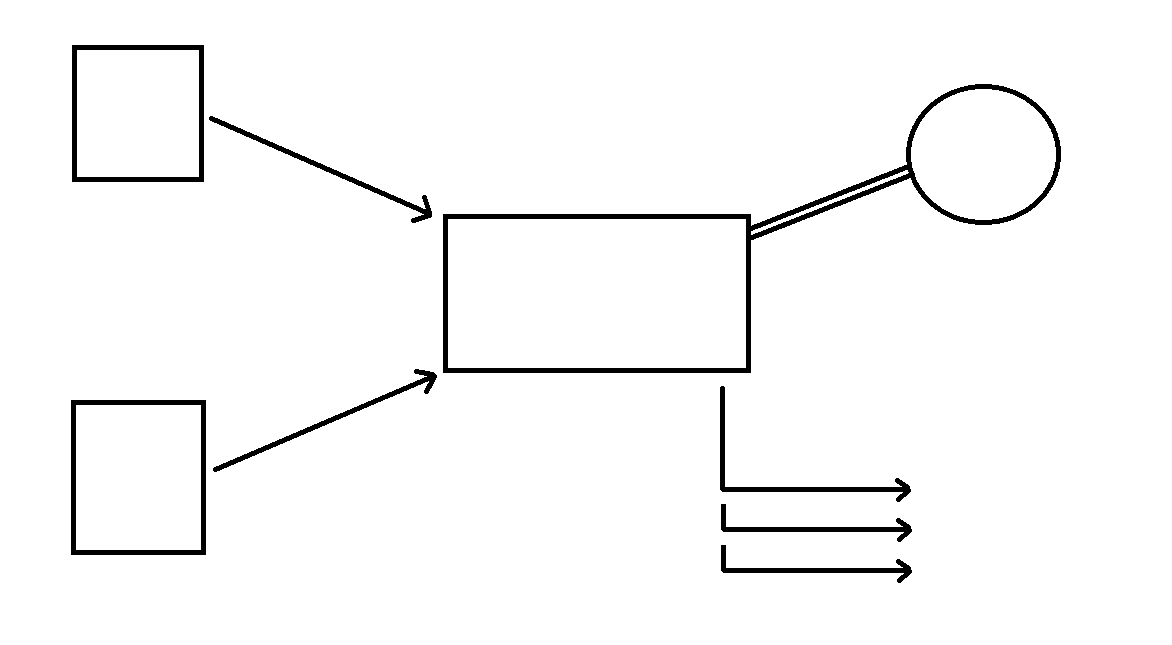
\includegraphics[height=8cm]{presentation/schema}
\end{center}
\caption[schema]{Presentation schema}
\end{figure}

\paragraph*{Paragraphe 1}
~\\
\hskip7mm

Bla

\paragraph*{Paragraphe 2}
~\\
\hskip7mm

Bla

\paragraph*{Paragraphe 3}
~\\
\hskip7mm

Bla

\newpage

%récupérer les citation avec "/footnotemark"
\nocite{*}

%choix du style de la biblio
\bibliographystyle{plainurl} %plain, ieeetr
%inclusion de la agsm
\bibliography{bibliographie.bib}
%voir wiki pour plus d'information sur la syntaxe des entrées d'une bibliographie

\end{document}